\documentclass[10pt, a4paper, twoside]{article}

% Set up the standard margins for the document
% 42.2 left & 15.5 right is same as Forsling, Neymark
% 21.3 top  & 20 bottom is same as Olofsson
\usepackage[left=25.5mm, right=25.5mm, top=21.3mm, bottom=20mm]{geometry}

% Input file character encoding (kinda useless if we don't
% use åäö and stuff, but it doesn't hurt to have it)
\usepackage[utf8]{inputenc}
%\usepackage[swedish]{babel}
\usepackage{caption}
\usepackage{subcaption}
% Block Comments
\usepackage{comment}

% No indentation in new paragraph
\usepackage{parskip}

% To include graphics
\usepackage{graphicx}

% More mathematical symbols and fonts
\usepackage{amsmath}
\usepackage{amsfonts}
\usepackage{amssymb}

% Simple list
\usepackage[ampersand]{easylist}
\ListProperties(Hide=100, Hang=true, Progressive=5ex, Style*=$\bullet$ ,
Style2*=-- ,Style3*=$\circ$ ,Style4*=\tiny$\blacksquare$ )


% Clickable internal links
\usepackage{hyperref}
\usepackage[all]{hypcap} % without this the link takes you to the caption, not the top of the image
\hypersetup{ % Settings for links in documnet
	setpagesize = false, % Don't allow hyperref to change page size. Tips från Micke Olofsson
	colorlinks = true,   % No boxes around links
	linkcolor = black,citecolor = black,filecolor = black,urlcolor = black, % don't color links
}

% To include to first page pdf file
\usepackage{pdfpages}

% Add section number to equation and figure number (ex: 5.11 instead of simply 11)
\numberwithin{equation}{subsection}
\numberwithin{figure}{section}
\numberwithin{table}{section}

% Show program code listings in document
\usepackage{listings}

%
% Header stuff
%
\usepackage{fancyhdr}
\setlength{\headheight}{15pt}

\fancyhf{}
\fancyhead[LE, RO]{\thepage}
\fancyhead[RE]{TSBB11 2013: System view}
\fancyhead[LO]{Kitchen Occupation}

\fancypagestyle{plain}{ %
\fancyhf{} % remove everything
\renewcommand{\headrulewidth}{0pt} % remove lines as well
\renewcommand{\footrulewidth}{0pt}}
%
% End header stuff
%


\begin{document}

% First page

\includepdf{Cover/cover.pdf}


% Project identity page
\newpage
\pagestyle{fancy}
\pagenumbering{roman}
\setcounter{page}{2} % sets the current page number to 2 

\begin{center}
    \vspace*{4\baselineskip}

	\textbf{\huge Project Kitchen Occupation} \\
	\vspace*{0.5\baselineskip}
	Bilder och Grafik CDIO, HT 2013 \\
	Department of Electrical Engineering (ISY), Link\"{o}ping University
	
	\vspace*{2\baselineskip}
	\textbf{\LARGE Participants}


	{\footnotesize 
	\begin{tabular}{|p{2.7cm}|p{1cm}|p{5cm}|p{2cm}|p{3.4cm}|}
		\hline
		\textbf{Name} & \textbf{Tag} & \textbf{Responsibilities} & \textbf{Phone} & \textbf{E-mail} \\
		\hline
		Mattias Tiger & MT & Project manager & 073--695\,71\,53 & matti166@student.liu.se \\
		\hline
		Erik Fall & EF & -- & 076--186\,98\,84 & erifa226@student.liu.se \\
		\hline
		Gustav Häger & GH & System integration & 070--649\,03\,97 & gusha124@student.liu.se \\
		\hline
		Malin Rudin & MR & -- & 073--800\,35\,77 & malru103@student.liu.se \\
		\hline
		Alexander Sjöholm & AS & -- & 076--225\,11\,74 & alesj050@student.liu.se \\
		\hline
		Martin Svensson & MS & Documentation & 070--289\,01\,49 & marsv106@student.liu.se \\
		\hline
		Nikolaus West & NW & Testing & 073--698\,92\,60 & nikwe491@student.liu.se \\
		\hline
	\end{tabular}
	}

{\footnotesize 
\vspace{0.5\baselineskip}
\textbf{Homepage}: TBA \\
\vspace{1\baselineskip}

\textbf{Customer}: Joakim Nejdeby, Link\"{o}ping University, Origo 3154 \\
\textbf{Customer contact}: 013--28\,17\,57, joakim.nejdeby@liu.se \\
\textbf{Project supervisor}: Fahad Khan, Link\"{o}ping University, fahad.khan@liu.se \\
\textbf{Examiner}: Michael Felsberg, michael.felsberg@liu.se \\
}

\end{center}



% table of contents
\newpage
\tableofcontents
\listoffigures
%\listoftables


% Document history page
\newpage
\vspace*{5\baselineskip}

\begin{center}
\textbf{\LARGE Document history}

{ \footnotesize 
\begin{tabular}{|p{1cm}|p{2.0cm}|p{5cm}|p{1.5cm}|p{2cm}|}
	\hline
	\textbf{Version} & \textbf{Date} & \textbf{Changes} & \textbf{Sign} & \textbf{Reviewed} \\
	
	\hline
	0.1 & 2013--09--10 & Initial draft & MS & \\
	\hline
	1.0 & 2013--05--24 & Final Document & All & \\
	
	\hline
	 &  &  &  &  \\
	
	\hline
\end{tabular}
}
\end{center}


% Blank page
%\newpage
%\thispagestyle{empty}
%\mbox{}

%
% Content start
%
\newpage
\pagenumbering{arabic}


\newpage
\section{Introduction}
\label{sec:introduction}
What to write here? maybe nothing.

\subsection{About this document}
This docment, is the user manueal....


\newpage
\section{Project Overview}
\label{sec:project_overview}
Text here.

\begin{figure}[htb]
	\centering
	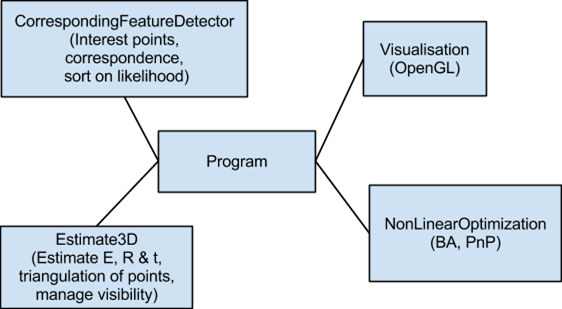
\includegraphics[width=110mm]{images/example2.png}
	\caption[This text ends up at the table of figures]{\textit{Image of entire system and its modules (THIS IS AN EXAMPLE IMAGE) }}
	\label{fig:block_overview2_fig}  %Skapar referens till figuren
\end{figure}

\subsection{Main program}
Text here.




\newpage
\section{Hardware}
\label{sec:hardware}

Since the system is to be able to run on two different platforms, the hardware requirements differ a lot depending on which system being considered. In the case of Raspberry Pi computers being used, all cameras each have their own Raspberry Pi processing unit where image processing takes place. In case of a central image processing unit (laptop, server or desktop computer), image processing from all cameras in the room take place on this central unit.


\begin{figure}[htb]
	\centering
	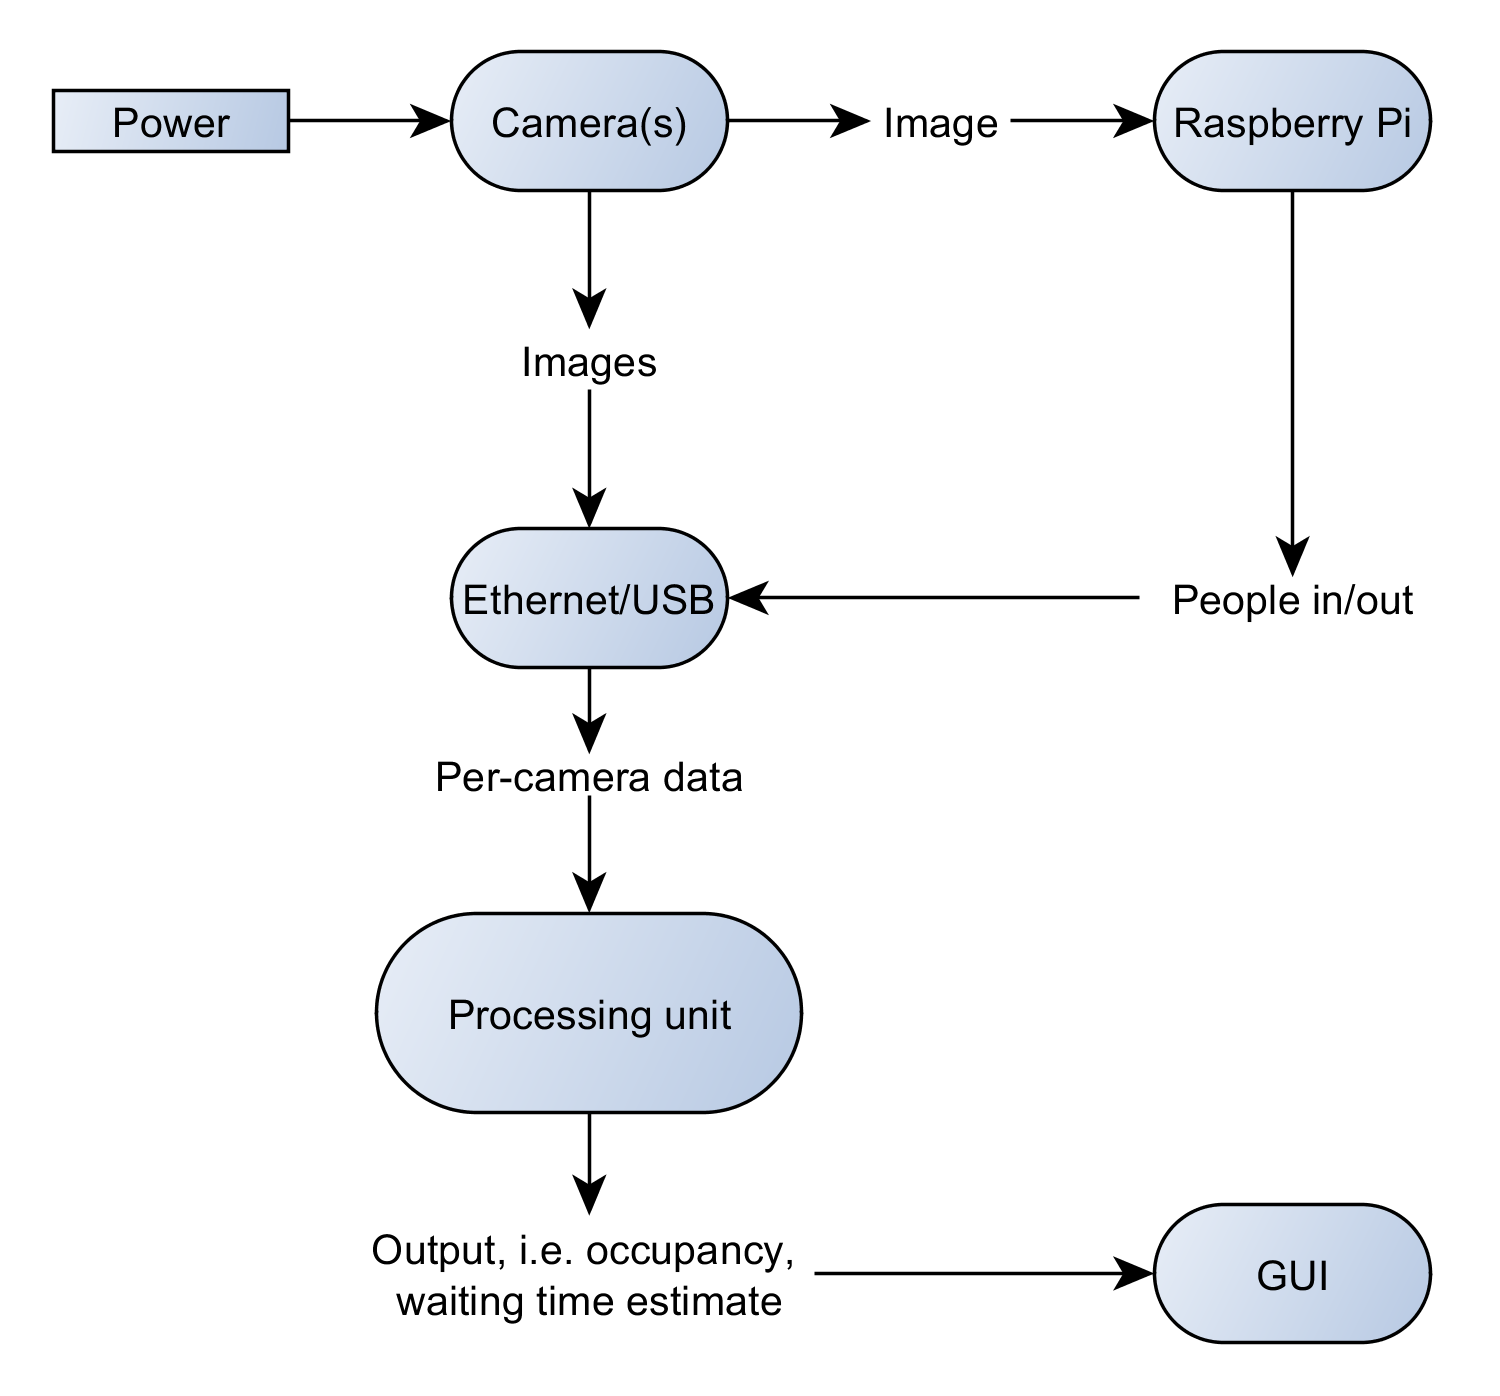
\includegraphics[width=160mm]{images/Hardware.png}
	\caption{\textit{Flowchart displaying data flow between hardware modules}}
	\label{fig:block_overview_fig}  %Skapar referens till figuren
\end{figure}
\newpage

\subsection{Limitations}
The hardware is limited by budget, Internet connection and the source of power. The cost is limited to approximately 15.000 SEK per room, including installation costs. The budget limits performance of the cameras e.g. resolution and number of cameras. The connection from the cameras to the processing unit(s) needs to be stable and have a bandwidth good enough for sending live video from the cameras. Additionally, no image data may be transmitted over public networks.   
\newpage
\subsection{Hardware Requirements}
\label{sec:hardware_req}
\reqtable
{
	\addreq{The system uses network cameras powered via Ethernet.\newline \textbf{Revised 2013-11-27:} The system uses cameras connected to a laptop (or similar mid-end processing device) via network or USB.}{1}	
	\addreq{The system can operate using high resolution ($>$2 Mpixel) cameras}{1}
	\addreq{Lower resolution cameras can be used}{2}
	\addreq{The application can run using the processing power provided by the costumer.\newline \textbf{Canceled 2013-11-27: }No processing power will be provided by the customer within the delivery time.}{--}
	\addreq{The application can run using a mid-end processing device (e.g. a laptop or desktop computer).\newline \textbf{Revised priority 2013-11-27:} The cancellation of previous req.(\textbf{3.4}) causes priority to change \textbf{from 2 to 1.}}{1}
	\addreq{The application can run using a low-end processing device.\newline	\textbf{Revised priority 2013-11-27:} Revised due to a request from customer that the system is able to run on a Raspberry Pi. Priority changed \textbf{from 3 to 2.}}{2}
}

\newpage
\section{Network module}
\label{sec:network_module}
Text.

\subsection{Camera API}
Text here

\subsection{Network communication}
Text here



\newpage
\section{Image processing}
\label{sec:image_processing}
Text here.

\subsection{Software}
Text here

\subsection{Tracking}
Text here

\subsection{Counting people}
Text here.


\newpage
\section{Estimation of waiting time}
\label{sec:estimate_time}
Text about this part of the system

\subsection{Queue detection}
Text here

\subsection{Mathematical models}
Text here

\subsection{Machine learning (?)}
Text here

\newpage
\section{User interface}
\label{sec:user_interface}
Text about the UI and result presentation.


\subsection{Presentation of results}
Text here

\subsection{Webpage}
Text here



% might not be necessary
\newpage
\section{Installation program}
\label{sec:install}
Text about the different deliveries and deadlines


\subsection{Milestones}
Text here

\subsection{Deliveries}
Text here



%
% Bibliography
%

% Force a blank page so the bibliography starts on a new page.
% Comment out if not necessary
%\newpage
\thispagestyle{fancy}
\mbox{}
\newpage
\begin{thebibliography}{9}
\addcontentsline{toc}{section}{References} % Add an entry for this in the table of contents

\bibitem{Gardel}
	Gardel, A., Bravo, I., Jimenez, P., Lazaro, J.L. \& Torquemada, A.\\
	``\textit{Statistical Background Models with Shadow Detection for Video Based Tracking},''\\ Intelligent Signal Processing, 2007. WISP 2007. IEEE International Symposium on?? Page: 1-6.
	
\bibitem{Zivkovic}
	Zivkovic, Z. \& Heijden, F.\\
	``\textit{Efficient Adaptive Density Estimation per Image Pixel for the Task of Background Subtraction},''\\
	Pattern recognition letters, Vol. 27, No. 7. (2006), pp. 773-780.

\vspace{2cm}
\LARGE{\textbf{EXAMPLE REFERENCES ONLY, REMOVE BEFORE HANDING IN}}
\normalsize
\bibitem{CVBook}
	Sonka, M., Hlavac, V. \& Boyle, R. 
	\emph{Image Processing, Analysis, and Machine Vision}.\\
	Toronto: Thompson Learning,
	cop. 2008, 3rd ed.,
	ISBN 0495244384.
	
\bibitem{Wood}
	Wood, J. (2007)
	``\textit{Statistical Background Models with Shadow Detection for Video Based Tracking},''\\
	Master thesis, Linköping University, Department of Electrical Engineering.	

\bibitem{DSPBook}
	Gustafsson, F., Ljung, L. \& Millnert, M.
	\emph{Signal Processing}.\\
	Studentlitteratur, Lund, Sweden,
	2011, 1st ed.,
	ISBN 978--91--44--05835--1.

\bibitem{MOTA}
	Bernardin, K. \& Stiefelhagen, R (2008)\\
	``\textit{Evaluating Multiple Object Tracking Performance: The CLEAR MOT Metrics},''\\
	Interactive Systems Lab, Institut für Theoretische Informatik,\\
	Universität Karlsruhe, 76131 Karlsruhe, Germany

\bibitem{CAVIAR}
	``\textit{CAVIAR: Context Aware Vision using Image-based Active Recognition},''\\
	EC Funded CAVIAR project/IST 2001 37540\\
	http://homepages.inf.ed.ac.uk/rbf/CAVIAR/
	

%\bibitem{somePaper}
%	Q. Lastname,
%	``Some article title,''
%	\emph{Some scientific journal},
%	vol.~1337, no.~1337,
%	pp.~666--1337,
%	month.~1337.

\end{thebibliography}



\end{document}
